\section{Primo approccio: modello lineare}

\subsection{Workspace}

Prima di iniziare a parlare del modello adottato per prevedere la richiesta di
\emph{Bike sharing}, è opportuno chiarire come verranno gestite le variabili
coinvolte durante l'analisi dei dati.

\subsubsection{Variabili esplicative}\label{sec:modlin-work-espl}
Per quanto riguarda le variabili esplicative, \texttt{holiday},
\texttt{working day}, \texttt{weather}, \texttt{temp}, \texttt{atemp},
\texttt{humidity}, \texttt{windspeed} non verranno trasformate in alcun modo.
In particolare:

\begin{itemize}
\item \texttt{holiday}, pur essendo qualitativa, è già espressa in un formato
  accettabile, ovvero \textbf{0} per una modalità (\textbf{N}) e \textbf{1}
  per l'altra (\textbf{S});
\item il caso di \texttt{workingday} è totalmente analogo a quello di
  \texttt{holiday};
\item \texttt{weather}, pur prevedendo quattro modalità, si può vedere come
  una variabile quantitativa per la quale più alto è il valore, peggiore è il
  tempo (con valori compresi tra quelli nominati nella sezione
  \ref{sec:intro-dati}).
\end{itemize}

\paragraph{Variabili trasformate} \mbox{}\\
Non tutte le variabili in gioco erano fornite in modo tale da essere
analizzate con semplicità.
Le restanti variabili esplicative sono state modificate con i seguenti criteri:

\begin{itemize}
\item \texttt{datetime} conteneva al suo interno il giorno e l'ora.
  Dopo una rapida analisi del dataset, si è notato che tutte le ore erano in
  realtà nel formato ``HH:00:00'', deducendo che si trattasse di misurazioni
  orarie. \\
  Oltre a ciò è stato considerato che la richiesta del servizio di \emph{Bike
  sharing} non dipende strettamente da un giorno particolare (e.g. 2012-07-04),
  ma principalmente dalla stagione a cui questo apparteneva e al fatto che
  questo fosse festivo e/o feriale o meno, fattori già presenti in altre
  variabili esplicative. \\
  A maggior ragione, lo scopo finale del modello era quello di effettuare
  previsioni su giorni non presenti nel dataset, perciò riuscire a costruire
  un modello che restituisse previsioni corrette su un giorno di cui si
  conoscevano già i risultati non era significativo, mentre il trend con cui
  il servizio viene richiesto durante una giornata potrebbe esserlo. \\
  Di conseguenza, si è ritenuto opportuno trasformare \texttt{datetime} in una
  variabile con valori interi uguali ad HH (ignorando completamente il
  giorno), con valori perciò compresi tra 0 (mezzanotte) e 23 (11:00 PM);
\item \texttt{season} presentava quattro possibili modalità. A differenza di
  \texttt{weather}, le cui modalità potevano essere viste come un insieme
  ordinato, non si vede alcun ordine per le stagioni. \\
  Un possibile tentativo sarebbe stato, in modo del tutto analogo a
  \texttt{weather}, pensare a un insieme dove al valore minimo sarebbe
  corrisposta la stagione caratterizzata da temperature più fredde e da
  condizioni metereologiche peggiori e viceversa per il valore massimo. \\
  Tuttavia, questo approccio non è stato considerato valido poichè primavera e
  autunno sono simili da questo punto di vista. \\
  Si è proceduto creando due nuove variabili, \texttt{season.summer} e
  \texttt{season.fall}, così che la variabile originaria \texttt{summer} fosse
  riorganizzata nel seguente modo:
  \begin{itemize}
  \item \texttt{season} variabile che vale 1 se la stagione è primavera
    (modalità \textbf{1} per la variabile originaria)
  \item \texttt{season.summer} variabile che vale 1 se la stagione è primavera
    (modalità \textbf{2} per la variabile originaria)
  \item \texttt{season.fall} variabile che vale 1 se la stagione è primavera
    (modalità \textbf{3} per la variabile originaria)
  \item  \texttt{season}, \texttt{season.summer} e \texttt{season.fall} con
    valore 0 se la stagione è inverno (modalità \textbf{4} per la variabile
    originaria)
  \end{itemize}
\end{itemize}

Tali trasformazioni sono state applicate durante il popolamento del dataset, il
cui script è stato riportato in sezione \ref{sec:script-populate}.

In fondo allo script si possono notare alcune costanti che vengono settate per
il workspace: si tratta di \texttt{columns}, ovvero i nomi delle variabili
esplicative utilizzate, e di altre costanti il cui uso verrà spiegato più
dettagliatamente in seguito.

\subsubsection{Variabili risposta}
Per le variabili risposta, è stato scelto di considerare solo
\texttt{train\$count}, poichè lo studio dei modelli per le variabili
\texttt{train\$registered} e \texttt{train\$casual} è del tutto analogo a
quello della variabile che insieme compongono.

%%%%%%%%%%%%%%%%%%%%%%%%%%%%%%%%%%%%%%%%%%%%%%%%%%%%%%%%%%%%%%%%%%%%%%%%%%%%%%%

\subsection{Modello lineare}\label{sec:mod-lin}
Dopo aver impostato correttamente il workspace, si può procedere calcolando il
modello lineare semplice $ y = \beta{}_0 + \beta{}_1 \cdot{} x + \epsilon{} $
per tutte le variabili, dove y è train\$count e x una delle variabili
esplicative.
Inizialmente questa operazione viene ripetuta con il comando \texttt{train.lm
= lm(y $ \sim{} $ x)} per tutte le variabili esplicative, ottenendo il
risultato migliore per x = train\$datetime.

Questo risultato ci può dare garanzie sulla buona intuizione riguardo il
formato scelto per la variabile \texttt{datetime}, spiegato nella sezione
\ref{sec:modlin-work-espl}, ovvero che l'ora è uno dei fattori che incidono
molto sulla richiesta del servizio di \emph{Bike sharing}.

Ci si aspetta infatti un andamento dicotomico della richiesta a seconda che
l'orario sia notturno (poca gente si muove di notte, ancor meno lo fa in bici)
o che sia diurno: sia i residenti che i turisti è più facile che si spostino di
giorno in bici per la città.

Tale considerazione può essere compresa guardando in figura
\ref{fig:simplest-linear-model} i valori dei residui visibili grazie alla
visione d'insieme del modello lineare fornita dal comando \texttt{summary()}.

\begin{figure}[H]
  \centering
  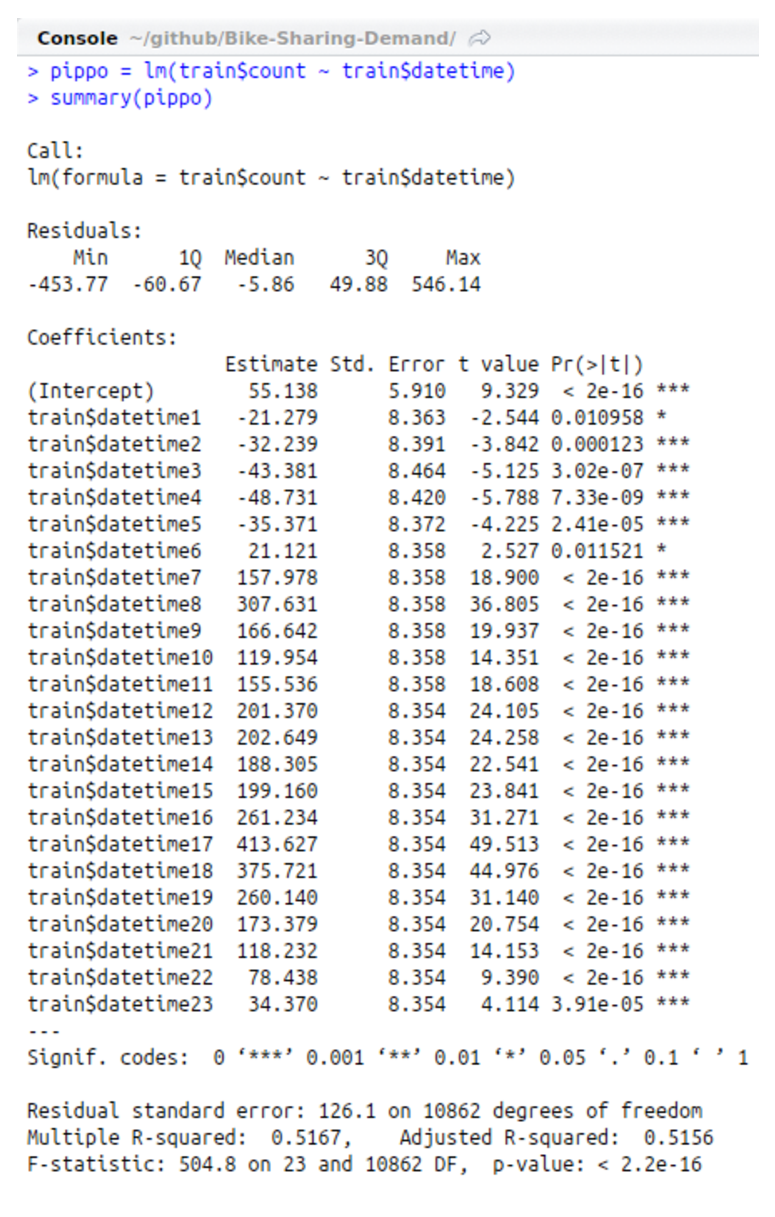
\includegraphics[width=.5\columnwidth]{images/lm/simplest-linear-model.eps}
  \caption{Modello lineare con \texttt{train\$datetime}}
  \label{fig:simplest-linear-model}
\end{figure}

I dati relativi al modello lineare appena individuato potrebbero ingenuamente
suggerire che la stima individuata per il coefficiente $\beta{}_1$ sia buona,
visto un valore molto elevato della statistica F e, di conseguenza, un p-value
prossimo a 0.

Tuttavia, vedendo il grafico dei residui di questo modello lineare (fig.
\ref{fig:simpl-mod-lin-residuals}), è ben facile intuire che il modello lineare
calcolato non è affatto soddisfacente, poichè è evidente che gli errori non
riescono a cogliere una curvatura presente nella risposta.

\begin{figure}[H]
  \centering
  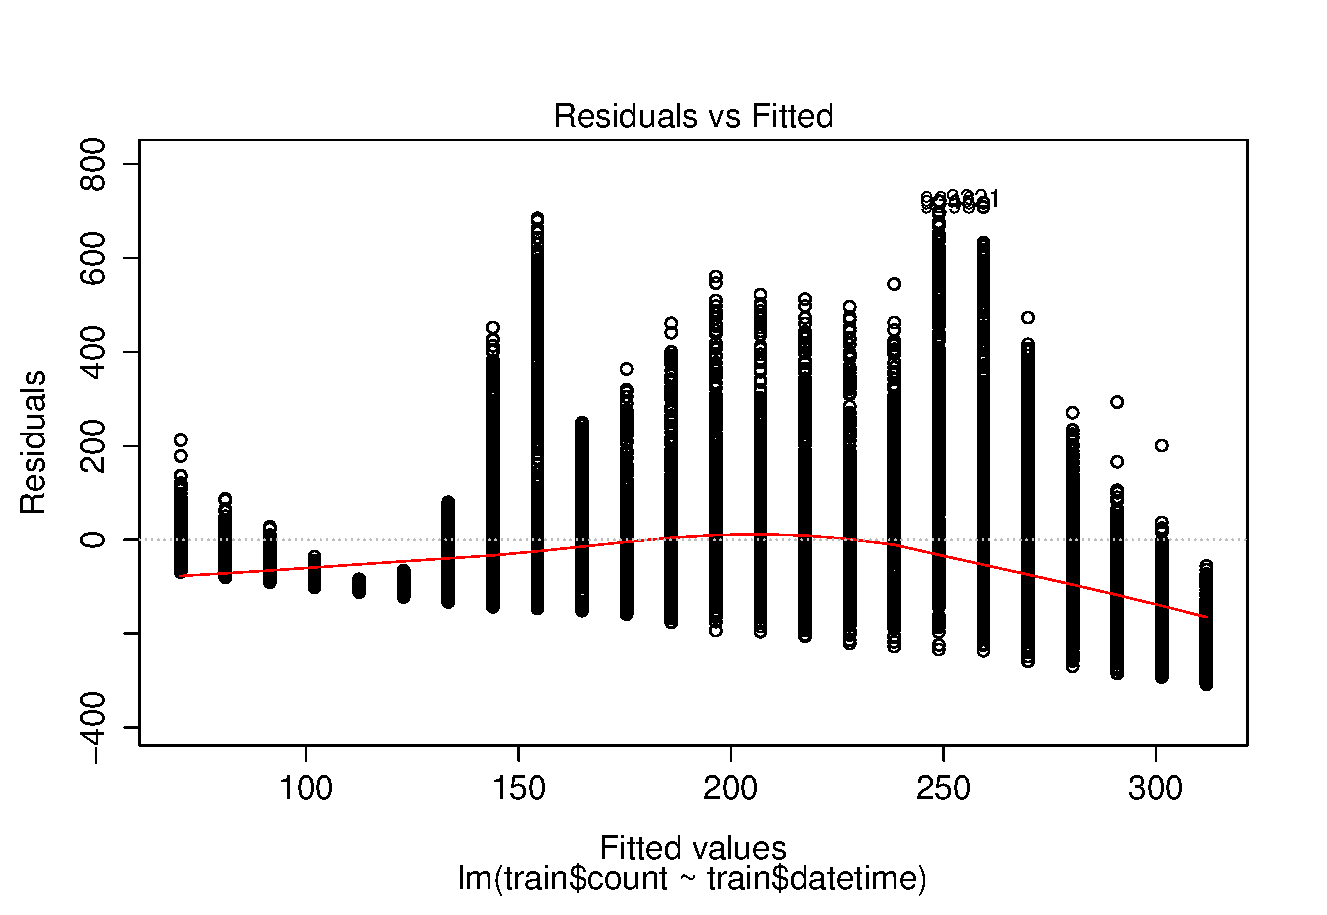
\includegraphics[width=.7\columnwidth]{images/lm/simple-linear-model-plot.eps}
  \caption{Grafico dei residui per il modello lineare con
  \texttt{train\$datetime}}
  \label{fig:simpl-mod-lin-residuals}
\end{figure}

\paragraph{Modelli con variabili esplicative trasformate} \mbox{}\\
Per rimediare a quanto detto sopra, si pensa a come introdurre nel modello
qualcosa che riesca a rappresentare nel modello la curvatura notata in figura
\ref{fig:simpl-mod-lin-residuals}.

Inizialmente il tentativo consiste nell'utilizzare un modello del tipo
$ y = \beta{}_0 + \beta{}_1 \cdot{} z + \epsilon{} $, dove z è la variabile
\texttt{train\$datetime} elevata al quadrato.

Come ci si può aspettare, questa strada però non porta i risultati desiderati:
nella figura \ref{fig:simpl-mod-lin-residuals} era ben visibile che le stime
``sbagliavano'' per eccesso (erano presenti molte sovrastime nel primo modello
lineare).

Perciò è totalmente naturale che elevando al quadrato la variabile esplicativa,
questo effetto negativo possa solo aumentare.

\paragraph{Modello con variabile risposta trasformata} \mbox{}\\
Si procede dunque con un secondo tentativo, provando ad agire sul valore della
variabile risposta. Dagli stadi di analisi precedenti ormai è chiaro che
l'errore commesso era dovuto ad alcuni valori della variabile risposta che
erano piuttosto elevati e non venivano spiegati dal modello.

Anzichè trasformare le variabili esplicative, quindi, è più conveniente
trasformare la variabile risposta in modo da attenuare i valori più alti di
questa:

\centering $ w = \beta{}_0 + \beta{}_1 \cdot{} x + \epsilon{} $
\flushleft dove $ w = log(y) $.

Questo modello risulta vincente, poichè l'errore standard dei residui passa da
126.1 a 1.381 (come visibile in fig. \ref{fig:simpl-lm-log-summary}) e il
grafico dei residui non presenta più curvature anomale e risulta più conforme
rispetto ad una distribuzione normale (vedi fig.
\ref{fig:simpl-lm-log-residuals}).

\begin{figure}[H]
  \centering
  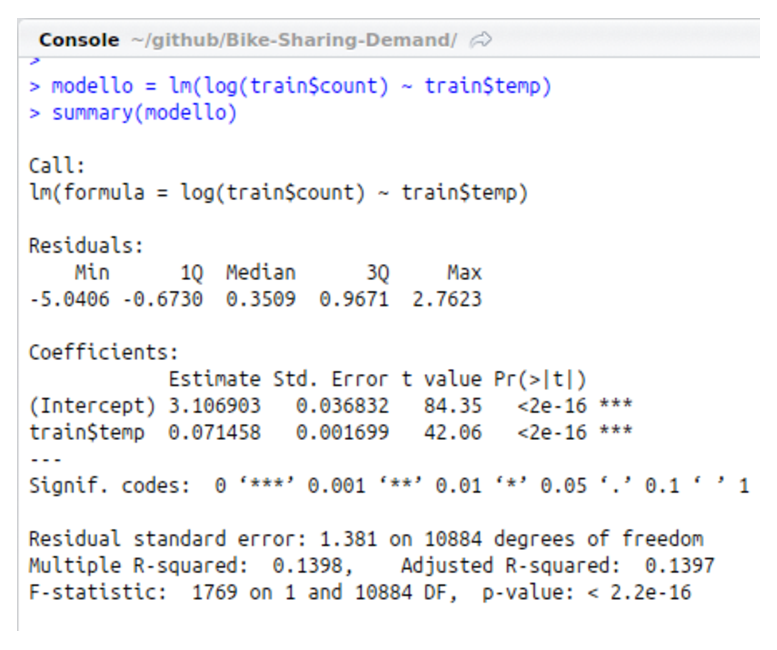
\includegraphics[width=.7\columnwidth]{images/lm/simpl-lm-summary.eps}
  \caption{Resoconto del modello con variabile trasformata}
  \label{fig:simpl-lm-log-summary}
\end{figure}

\begin{figure}[H]
  \centering
  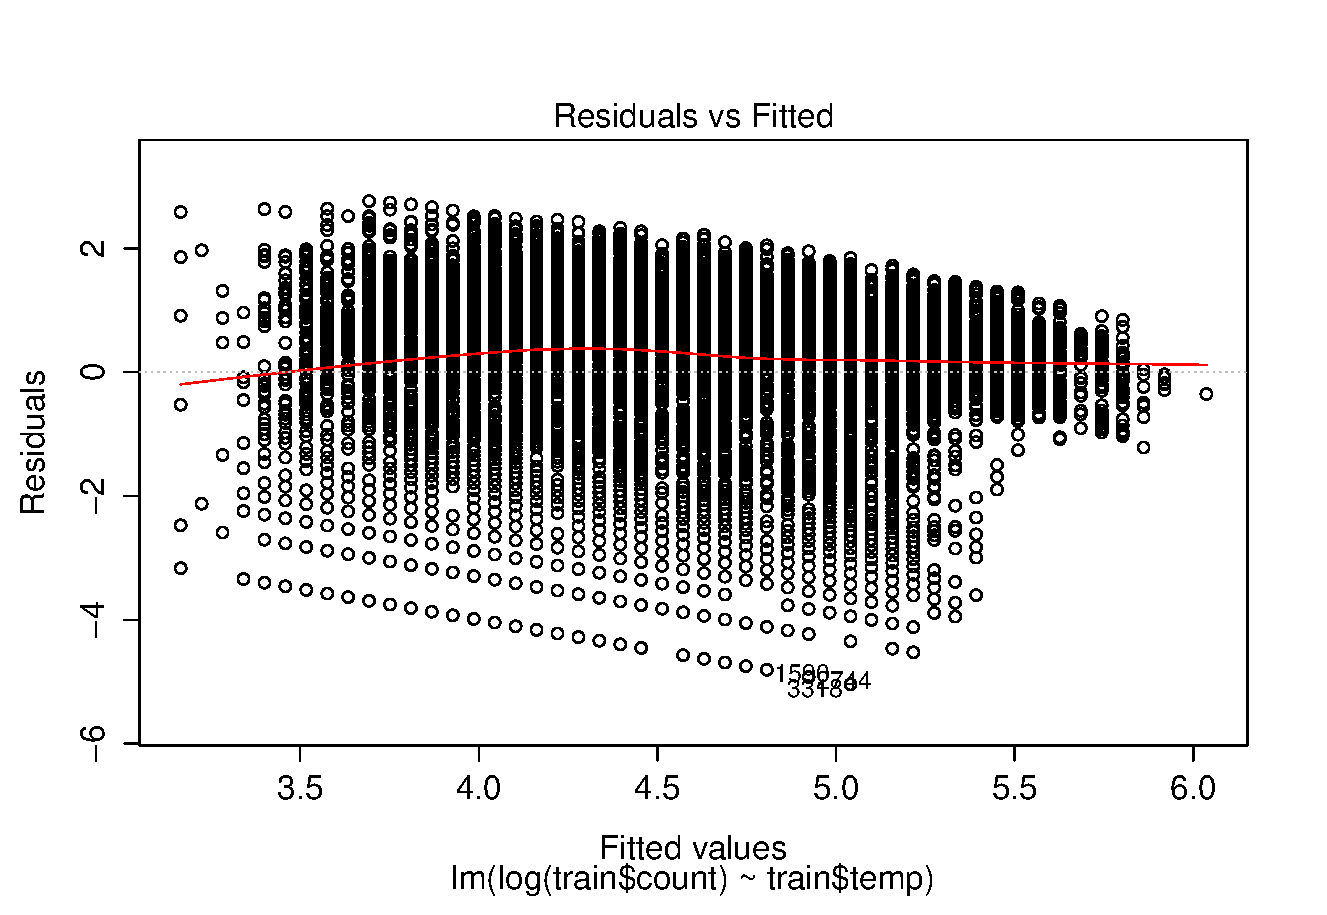
\includegraphics[width=.7\columnwidth]{images/lm/simple-lm-log-residuals.eps}
  \caption{Grafico dei residui con variabile trasformata}
  \label{fig:simpl-lm-log-residuals}
\end{figure}

%%%%%%%%%%%%%%%%%%%%%%%%%%%%%%%%%%%%%%%%%%%%%%%%%%%%%%%%%%%%%%%%%%%%%%%%%%%%%%%

\subsection{Modello lineare con \emph{forward stepwise selection}}\label{sec:mod-lin-fwd-sw}
Il modello di prima ha portato a discreti risultati, però utilizzava solamente
una delle variabili esplicative.

Un approccio naïf potrebbe essere quello di inserire nel calcolo del modello
lineare tutte le variabili esplicative presenti nel set \texttt{train} e di
calcolare il modello lineare con il comando fornito da R.

Come è possibile vedere in figura \ref{fig:simpl-lm-log-qqplot}, ci sono
alcune variabili che sono poco significative e altre che invece è sensato che
appartengano al nostro modello.

\begin{figure}[H]
  \centering
  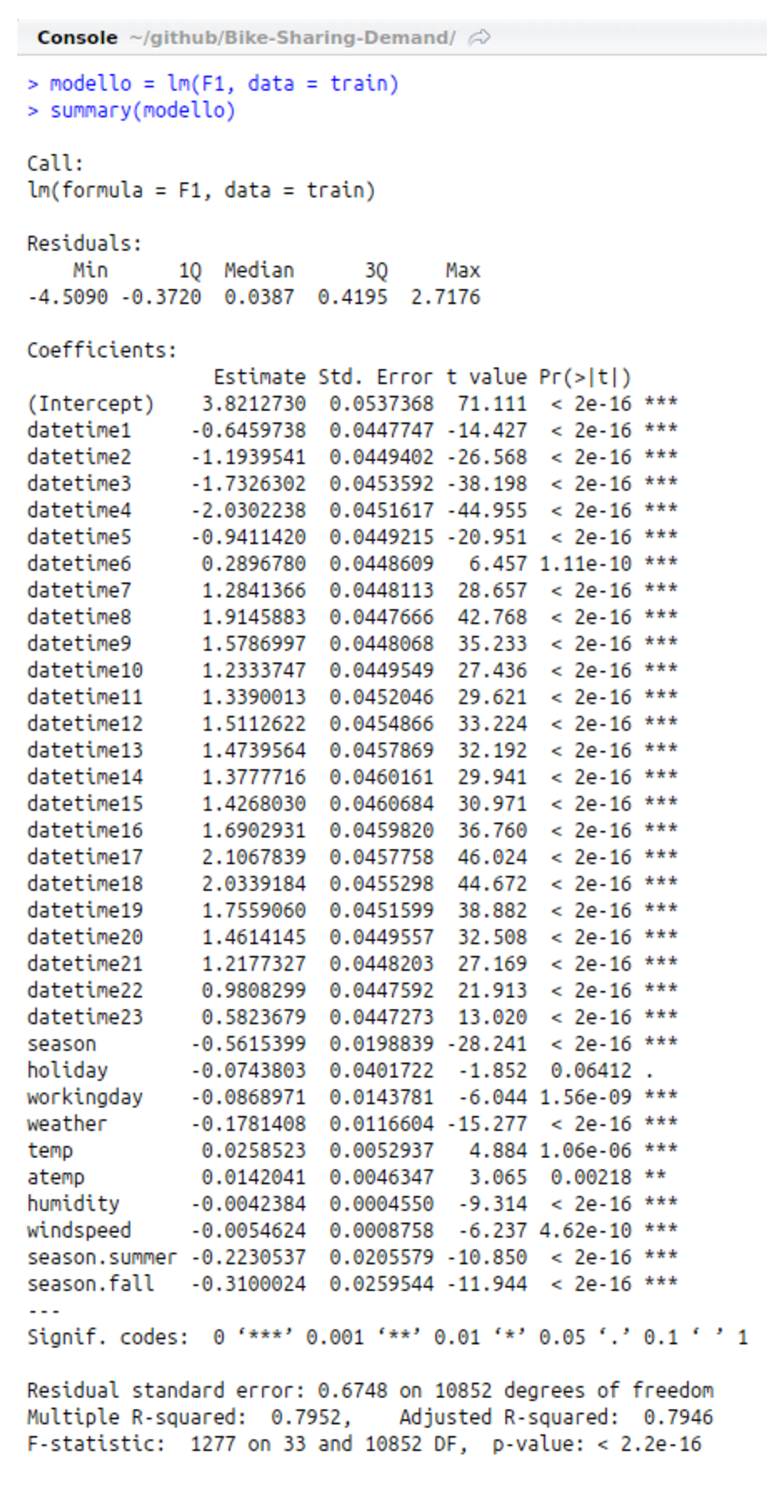
\includegraphics[width=.55\columnwidth]{images/lm/lm-with-all-vars.eps}
  \caption{Modello lineare calcolato su tutte le variabili}
  \label{fig:simpl-lm-log-qqplot}
\end{figure}

Tuttavia non sappiamo se potremmo togliere qualche variabile che potrebbe
essere significativa solamente per l'ordine in cui è stata inserita, o se la
variabile \texttt{holiday} possa essere trascurata per il nostro modello.

Tale variabile sembrerebbe significativa, poichè ci si aspetta che nei giorni
di festa vi sia più traffico in città (i dati sono relativi a Brooklyn) e che
la richiesta di \emph{Bike sharing} aumenti per evitare lunghe code in
macchina.

Anzichè provare manualmente qualsiasi combinazione di variabili fino a quando
non viene trovato il modello lineare migliore, si decide di automatizzare il
tutto con un paio di script (\texttt{linearModel.R} in sez.
\ref{sec:script-linear-model}, \texttt{linear\_model\_forward\_steps.R} in
sez. \ref{sec:script-linear-model-fwd-steps}) che implementano la regressione
lineare con \emph{forward-stepwise selection} penalizzando l'utilizzo di più
variabili tramite il criterio di Aikake.

Di seguito vengono riportati i dati del modello lineare ottenuto tramite gli
script sopra descritti:

\begin{figure}[H]
  \centering
  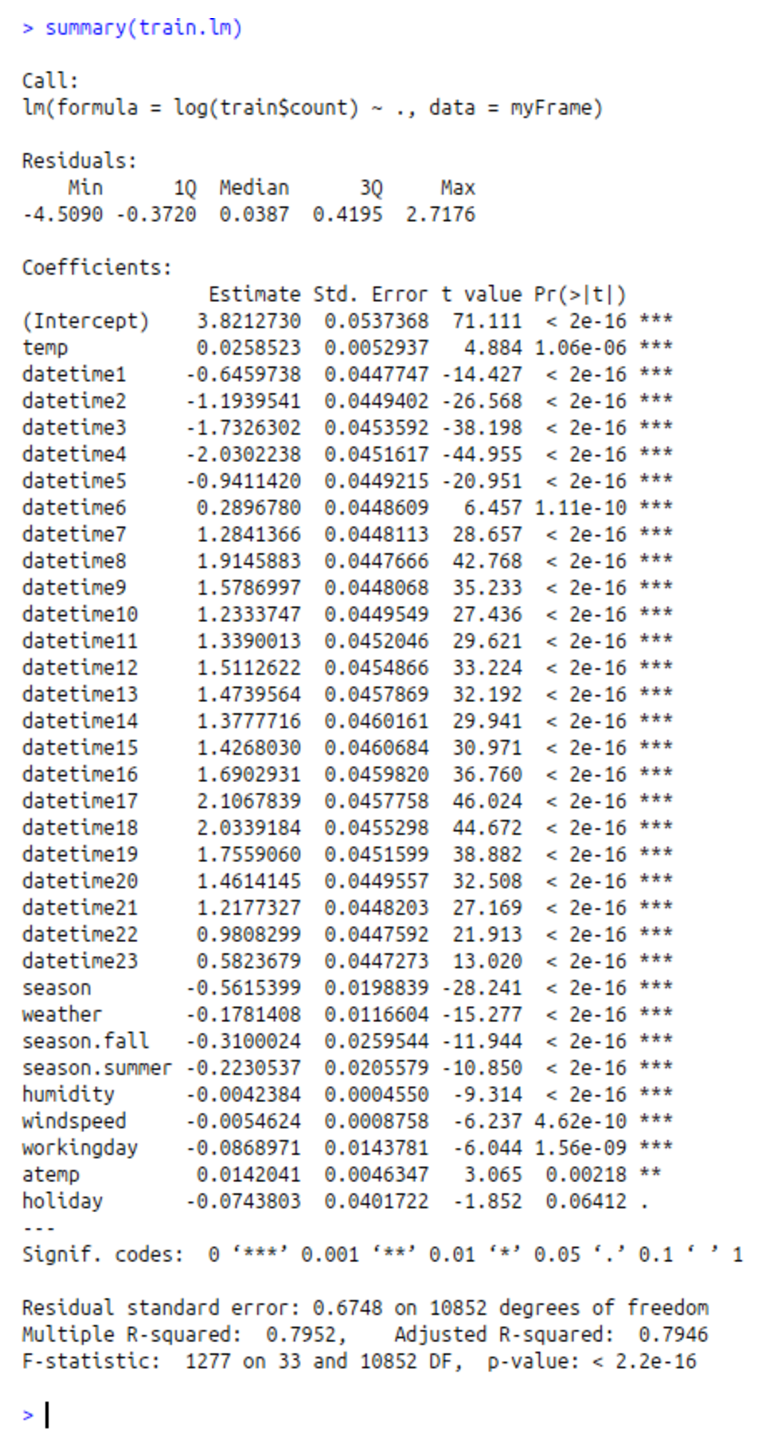
\includegraphics[width=.55\columnwidth]{images/lm/lm-after-fwd-steps.eps}
  \caption{Modello lineare calcolato tramite forward-stepwise selection}
    \label{fig:lm-after-fwd-steps}
\end{figure}

Come è possibile vedere nella seguente figura, i residui sono molto
soddisfacenti e sono sparsi intorno allo zero abbastanza uniformemente.

\begin{figure}[H]
  \centering
  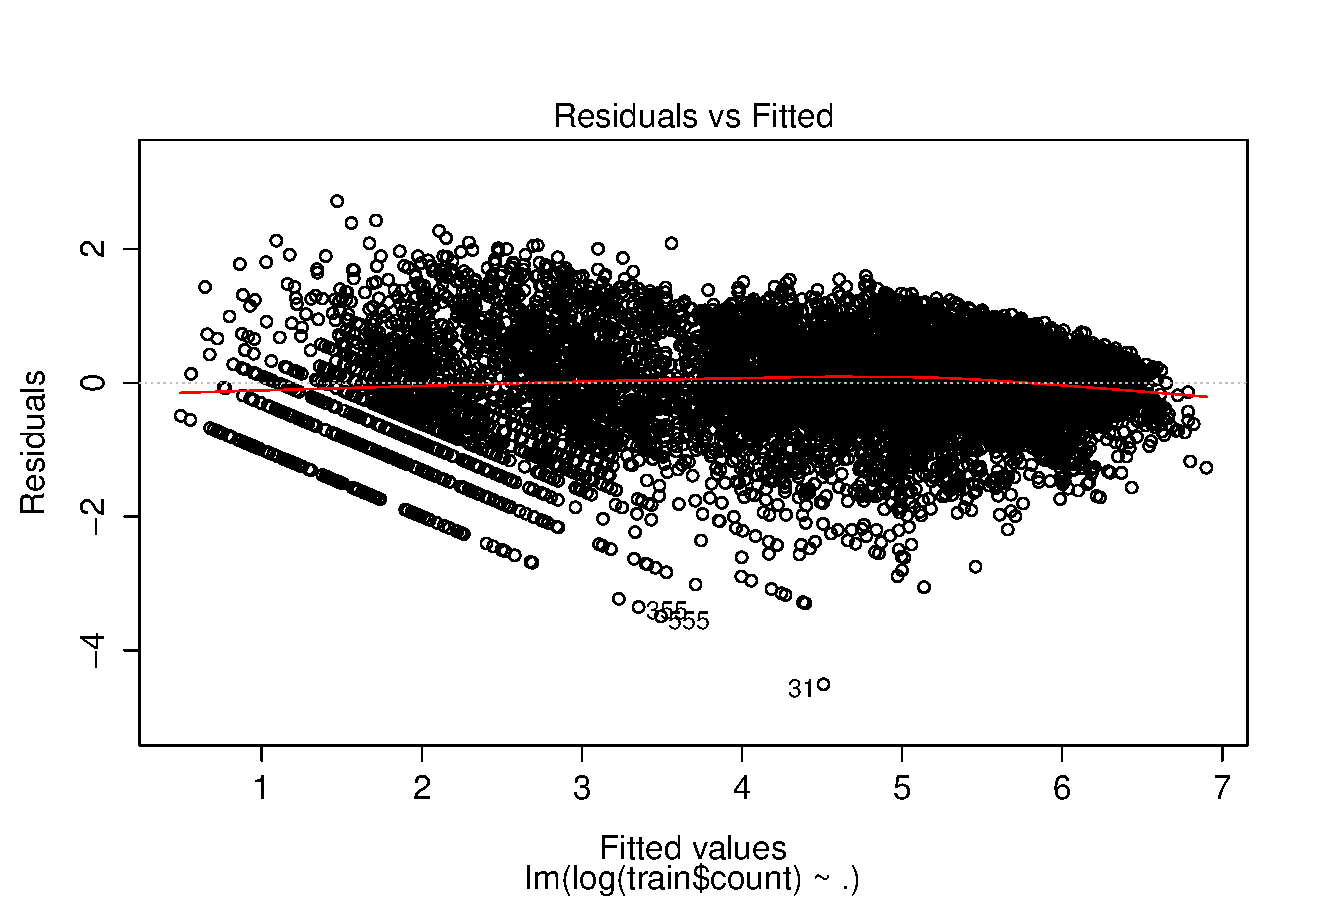
\includegraphics[width=.55\columnwidth]{images/lm/fwd-sw-residuals.eps}
  \caption{Modello lineare calcolato tramite forward-stepwise selection}
    \label{fig:fwd-sw-residuals}
\end{figure}

Il risultato non ci sorprende, siccome ci si aspettava che tutte le variabili
apportassero un contributo significativo per la richiesta del servizio; in
particolare, è possibile vedere la loro importanza in base all'ordine con cui
sono state inserite nel modello.

Tale procedura è stata applicata anche ai valori della variabile risposta in
scala originale, ottenendo i seguenti risultati:

\begin{figure}[H]
  \centering
  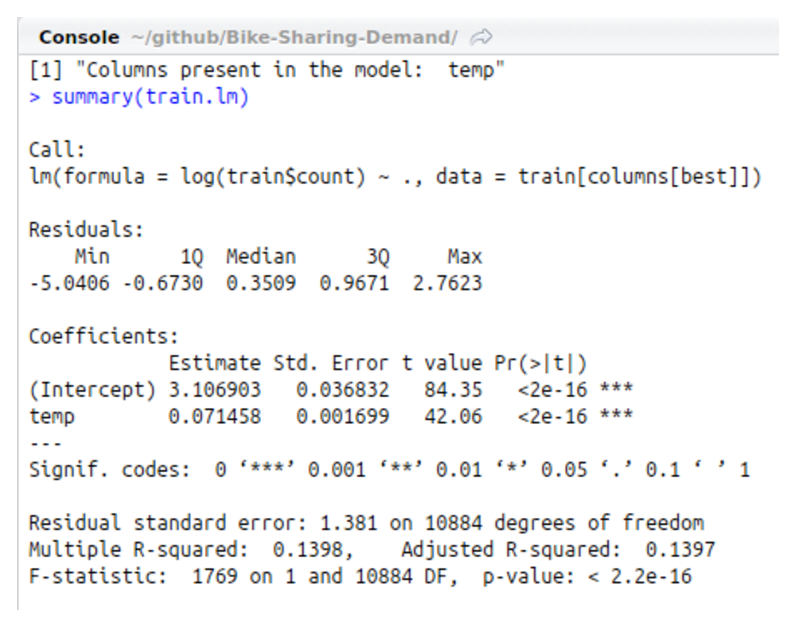
\includegraphics[width=.55\columnwidth]{images/lm/fwd-sw-nolog.eps}
  \caption{Modello lineare in scala originale calcolato tramite
    forward-stepwise selection}
    \label{fig:lm-after-fwd-steps-nolog}
\end{figure}

\begin{figure}[H]
  \centering
  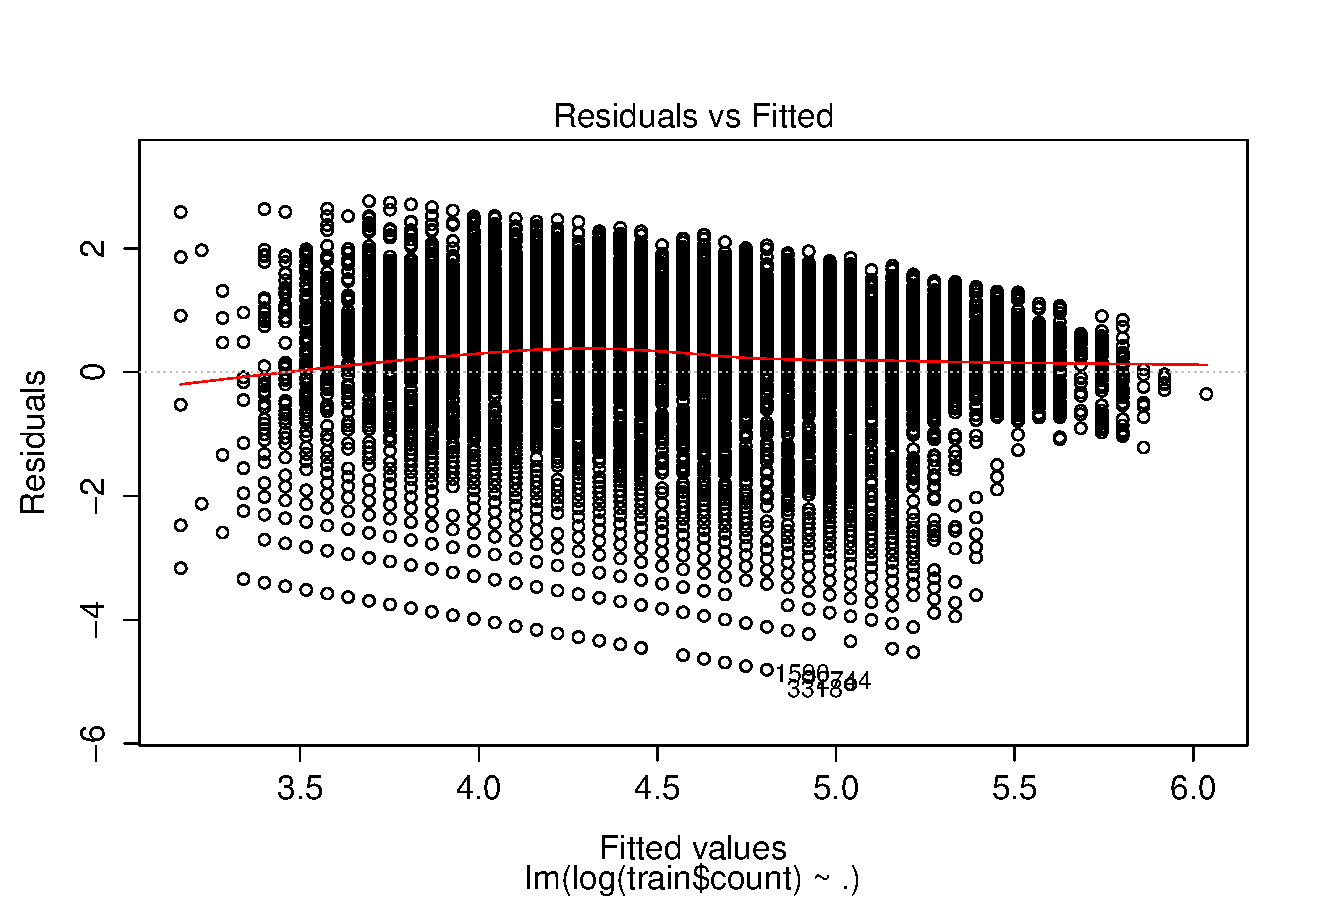
\includegraphics[width=.55\columnwidth]{images/lm/fwd-sw-nolog-residuals.eps}
  \caption{Modello lineare calcolato tramite forward-stepwise selection}
    \label{fig:fwd-sw-residuals}
\end{figure}

Un po' a sorpresa, nella scala originale i dati sono spiegati solamente dalla
variabile \texttt{temp}.

Tuttavia questo è ritenuto possibile poichè abbiamo visto prima che la
regressione lineare, per questi dati, in scala originale non coglie tutte le
variazioni della richiesta del servizio e approssimando l'intero modello ad
una retta con una sola variabile esplicativa.

%%%%%%%%%%%%%%%%%%%%%%%%%%%%%%%%%%%%%%%%%%%%%%%%%%%%%%%%%%%%%%%%%%%%%%%%%%%%%%%

\subsection{Stima ai minimi quadrati con filtro ricorsivo}
Anche se non richiesto dal problema, si è voluto rendere il calcolo del
modello lineare efficiente nel caso in cui il dataset non fosse composto da un
insieme di dati prefissati, ma da uno stream che continuasse a far pervenire
dati.

A tal riguardo è stato sviluppato uno script chiamato \texttt{KalmanFilter.R}
che lavora grazie a ortogonalizzazioni successive.

Tale algoritmo può essere paragonato ad un filtro di Kalman poichè anch'esso
cerca di valutare lo stato (più specificatamente, la relazione tra le
variabili esplicative e quella risposta) di un sistema dinamico (assumendo che
i dati arrivino tramite stream) le cui osservazioni si assume che siano
incorrelate, con distribuzione normale e a media nulla.

Oltre a ciò, ci si aspetta che la richiesta del servizio di \emph{Bike sharing}
segua un modello ``vero'', costante nel tempo e non casuale. In poche parole,
ci si aspetta che i vari valori $ \beta{}_i $ (dove $i$ è un indice relativo
alle variabili esplicative) abbiano stabilità asintotica.

Di seguito vengono riportati i coefficienti di $ \beta{} $ che, se confrontati
con quelli in figura \ref{fig:lm-after-fwd-steps}, ci convincono che il filtro
ricorsivo abbia funzionato correttamente.

Oltre a questi coefficienti, vengono riportati i grafici in cui è possibile
vedere che i valori in $ \beta{} $ raggiungono i valori ``veri'' per numerosità
di osservazioni sufficientemente elevate.

%%%%%%%%%%%%%%%%%%%%
%%% TODO
%%% 
%%% RIFARE FIGURE
%%%%%%%%%%%%%%%%%%%%

\begin{figure}[H]
  \centering
  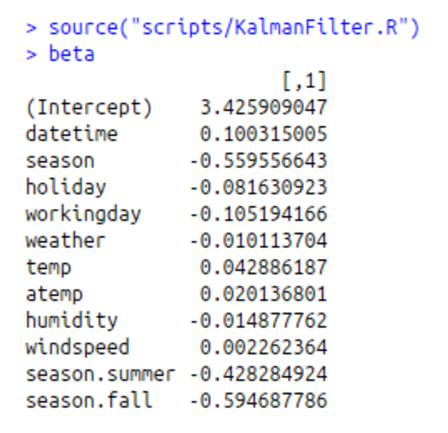
\includegraphics[width=.55\columnwidth]{images/lm/kalman-beta.eps}
  \caption{Coefficienti calcolati tramite filtro ricorsivo}
    \label{fig:kalman-beta}
\end{figure}

\begin{figure}[H]
  \centering
  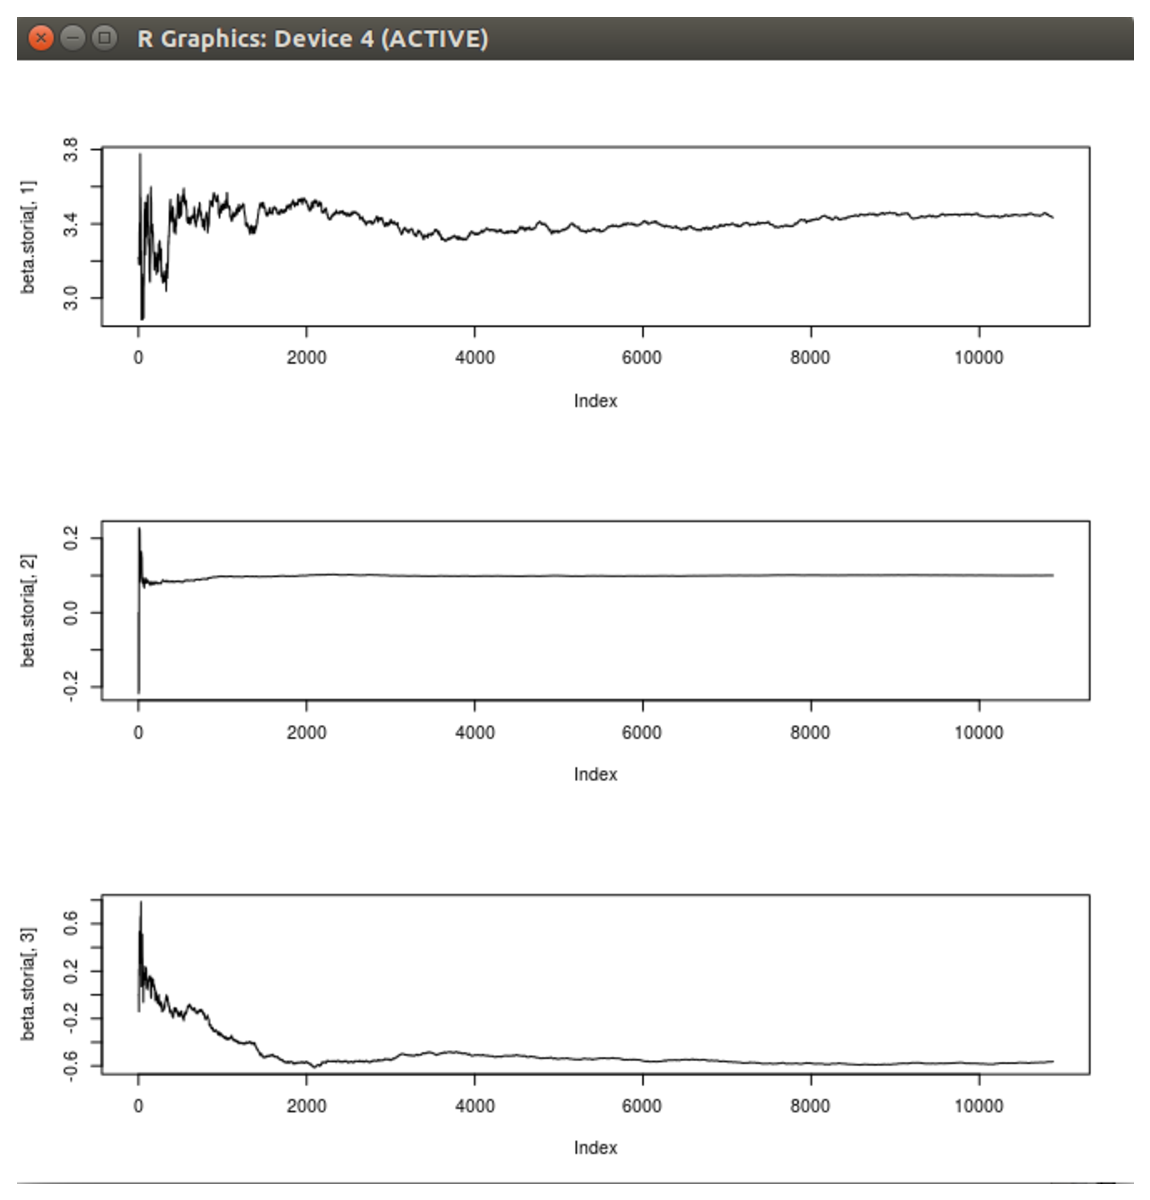
\includegraphics[width=.55\columnwidth]{images/lm/kalman-asymptotic.eps}
  \caption{Stabilità asintotica del filtro ricorsivo}
    \label{fig:kalman-asymptotic}
\end{figure}
